%max: 5pages

\documentclass{llncs}
%
\usepackage{makeidx}  % allows for indexgeneration
\usepackage{graphicx} % for photos
\usepackage{wrapfig}

%
\begin{document}
%
\frontmatter          % for the preliminaries
%
\pagestyle{headings}  % switches on printing of running heads
\addtocmark{Hamiltonian Mechanics} % additional mark in the TOC
%

\mainmatter              % start of the contributions
%
\title{Zone-project: towards a better news feed using semantic web}
%
\titlerunning{Zone-project}  % abbreviated title (for running head)
%                                     also used for the TOC unless
%                                     \toctitle is used
%
\author{Christophe Desclaux\inst{1}, Ameni Bouaziz \inst{2}\and Fabien Gandon \inst{1}}
%
\authorrunning{Christophe Desclaux} % abbreviated author list (for running head)
%
%%%% list of authors for the TOC (use if author list has to be modified)
\tocauthor{Christophe Desclaux}
%

\institute{Wimmics - Inria, Sophia Antipolis,\\
\email{christophe@zouig.org}\\
\url{http://www.zone-project.org}
\and
Université Nice Sophia Antipolis,\\
\email{bouazizamani@gmail.com}
}


\maketitle

\begin{abstract}%
The zone project proposes an innovative solution to address the traditional issues of news feed management using the resources of Semantic Web to group related informations together.
It provides a new way to follow feeds by aggregating items from various news feeds, tagging and annotating each one of them. Those tags provide a basis for filters allowing users to see only relevant news for her.

%The abstract should summarize the contents of the paper
%using at least 70 and at most 150 words. It will be set in 9-point
%font size and be inset 1.0 cm from the right and left margins.
%There will be two blank lines before and after the Abstract. \dots
\keywords{linked data, data aggregation, RSS}
\end{abstract}
%
\section{Motivation}
%
An important amount of news and data are published every day on the internet and the number of news websites has increased significantly. The abundance of theses sources able people and organisation to access a incredible knowledge database. More and more people are facing the same issue, how to retrieve, gather, organize and filter these sources in order to retrieve only the pertinent information?

Solutions exist, for instance one can use \textsl{Google news} \footnote{\url{http://news.google.fr}} like a trusted provider of information. This service can be very helpful but in practice limitations appears, you are only a consumer and you can't have many interaction with the service proposed.

A second kind of solutions is to make news forecasting using for instance \textsl{Twitter}\footnote{\url{http://www.twitter.com}}. It's a solution in which one can control the sources he follows. But you can't select precisely on sources and on topics at the same time and a lot of noise remains around good information. Even the hash-tags provide a limited solution since they suffer from collision.  

The last family of relevant solutions one can use is aggregators like \textsl{Yahoo Pipes} \footnote{\url{http://pipes.yahoo.com/pipes/}}. This service allows merging popular data feeds and data filtering using a visual editor. Pipes are then defined as workflows to help users to sort feeds. It's a good solution for specialists of news forcasting but is to difficult to use for non specialist public.

From these three kind of approaches, different important challenges can be identify:
\begin{itemize}
  \item \textbf{filtering capabilities}: select and sort information according to precise criteria;
  \item \textbf{open pool sources}: access a maximum of news present on internet and allow users to add new ones;
  \item \textbf{independence}: propose a solution independent from a service providers.
\end{itemize}

Solutions exists to overcome these challenges; Google solves the filtering problem using PageRank and search by keywords \cite{page:brin} however this method is not efficient as it works on words rather than working on meaning. The Zone project proposed in this paper aim to build a solution based on aggregation approach and semantic web framework where users are not only consumers but built an important database of news and share their filtering results.

In the following section, this paper describes our solution called Zone. We will explain the annotation workflow, the ontology used and the use of data-mining solutions. We will also present the scenario of the demonstration of the application.

%
\section{Application: Zone}


\subsection{The workflow}
%
\begin{figure}[htb!]
	\begin{centering}
	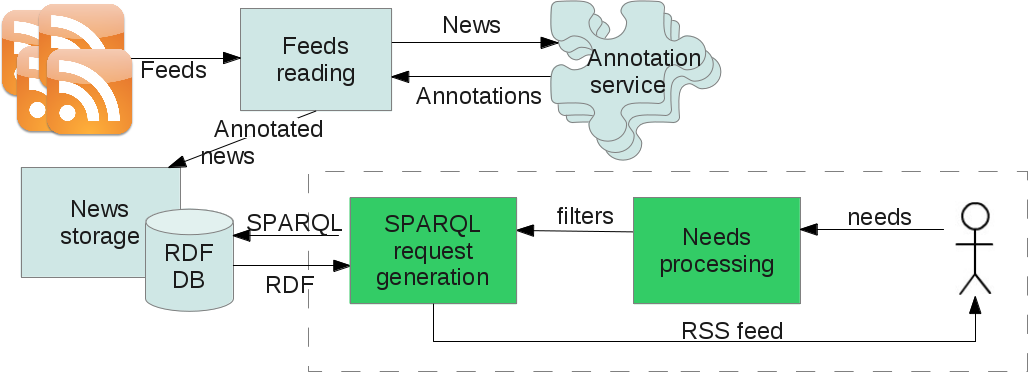
\includegraphics[width=1\textwidth]{diagram.png}
	\caption{Annotation workflows and semantic filtering of news}
	\label{fig:WF}
	\end{centering}
\end{figure}

In order to improve news selection according to their semantic relevance, two kinds of workflows are proposed. Figure \ref{fig:WF} shows the general architecture: a semantic annotation workflow of news and a filtering workflow. The distinction between these two workflows is extremely important as processes needs to work in an asynchronous way \cite{desclaux:urli}.

\subsubsection{The semantic annotation workflow.}
First, Zone crawls the web extracting news and storing them in database.

Two annotators extract semantic annotations from the textual content of the news: the first one is called Wikimeta \footnote{\url{http://www.wikimeta.com}}. It allows our system to create links to Wikipedia resources. The second one is called OpenCalais \footnote{\url{http://www.opencalais.com}} and provides geographical references.
The system also use others RDF database surch as DBpedia \footnote{\url{http://dbpedia.org}} and INSEEGeo \footnote{\url{http://rdf.insee.fr/geo}} in order to add more annotations for some elements (countries, people...).

News content and semantic annotations are stored together in a triple store (Virtuoso \footnote{\url{http://virtuoso.openlinksw.com}}). 


 
\subsubsection{The filtering workflow.}
Users can then access their data categorized by the annotation workflow. The results are concentrated in a web application using the web framework RubyOnRails. Users build filters that are stored and applied as SPARQL queries. These queries are then performed over the triple store fed by the annotation workflow. Finally, these results queries can be published by any users as a RSS feed containing only relevant news.

%
\subsection{The Zone-project News Ontology}
The work to formalize the ontology used to store news has been done reusing a maximum of other ontology. 
First we have take a look at news ontologies such as NewsML \footnote{\url{http://www.iptc.org/site/News\_Exchange\_Formats/NewsML-G2/}}. It' a solution held by news agencies to address datas in a semantic context. But this ontology was not efficient in our context, we decided to use a smaller one RSS \footnote{\url{http://web.resource.org/rss/1.0/spec}} which is much more used in news web services and which is an important part of our input news format. 

On top news are stored under the RSS formalism, annotations are stored under the Wikimeta \cite{charton:nlgbase} and
 OpenCalais \footnote{\url{http://www.opencalais.com/documentation/opencalais\-web\-service\-api/calais\-ontology\-owl}} ontologies and we added markers on each news in order to say if a news has already been annotated for a specific annotator. The sources followed by the system are also stored on the triple store in order to enable the annotators to use them. Finaly the draft of the ontology is published on \url{http://ns.inria.fr/zoneproject/}.
% graph of the ontology
% publish on ns.inria.fr 
% textual description of core classes and properties.

%**************basée sur RSS
%on a ajouté un schéma RDFs spécialisé
%on se base aussi sur l'ontologie de wikimeta/insee***************
%

%
\subsection{Using datamining}

In order to introduce data mining in our classification process, we decided to use a supervised learning algorithm based on the support vector machine (SVM). SVM are binary classifiers which analyse data and recognize patterns based on a learnt model with a set of training data. Given two categories, SVM construct a hyperplane that separates them.

SVM Light library \cite{joachim:svmlight} is used in our project for the classification. SVM light offers a learning step that construct the classification model starting from the set of training data and a second step to do the real classification based on the previously constructed model.

These two steps take as entry a feature vector which is prepared during the preprocessing step. For preprocessing phase we used Stanford CoreNlp libraries \footnote{\url{http://nlp.stanford.edu/software/corenlp.shtml}} and  Java code for stop words removing (punctuation, common words like I, he, she, what, have, be …).
Lemmas obtained are used to build a dictionary of all known words. Then we use TF-IDF algorithm to calculate the weight of each known lemma in the texts. The feature vector is afterwards built as pairs of rank of the lemma in the dictionary and its weight.

Thanks to our first successfully results made on the English test corpus "Reuters 21578" \cite{lewis:reuters}, we tested the algorithm on the 10 most important categories (money-fx, earn, acq, grain, crude, trade, interest, ship, wheat, corn) the recall obtained on the corpus varied from 0.63 to 0.96 depending on the category.

Then algorithm was adapt to work on french text classification in order to be integrated in ZONE. As validation corpus, we considered 5 categories (sport, economy, science, health and computer science). These categories were filled by RSS feeds specialized in each category and we split this data in a learning and a test corpus. A SVM classifier was created for each category and the classification was made on the test corpus. The recall obtained on this validation corpus reached 0.97 for the sport category which is the best represented in the training set. Then we obtain 0.78 for computer science and 0.52 for health. The values obtained for economy and science were too low, the small size of the training set may explain these values.
\begin{wrapfigure}{l}{0.48\textwidth}
  %\begin{left}
  \vspace{15pt}
	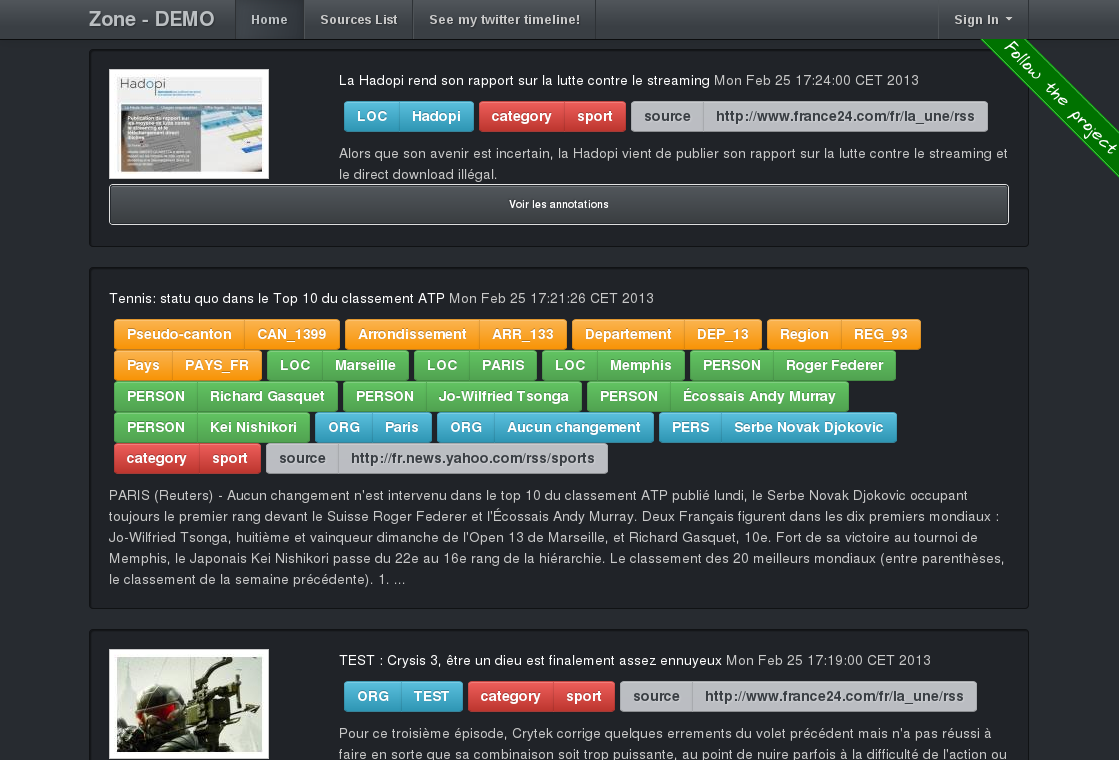
\includegraphics[width=0.48\textwidth]{zone-screenshot.png}
	%\caption{Capture of zone project solution}
	\label{fig:DEMO}
  %\end{left}
  \vspace{-60pt}
\end{wrapfigure}

\section{Demonstration}
%
The web application is designed for all kinds of news feeds like technology, medicine or general news. You can install the application according to your needs under the AGPL licence \footnote{\url{https://github.com/descl/ZONE}}. An experimental platform is also provided for general news feed at \url{http://demo.zone-project.org}.


The demo will start with the listing of all recent news on \url{http://demo.zone-project.org}. Then we will create a filter according to some criteria in order to show to the audience the different kinds of filters present and their links to the news. Once the good filter is chosen, we will show how to export it as an external RSS feed aggregator demonstrating that our web application can be used in combination to other tools.

Last, we will propose another use of ZONE-project based on Twitter. With another demo application we will make a quick demonstration of news filtering on the hashtag \#eswc2013.

\section{Conclusion and future work}
%
The goal of our demonstration is to show an efficient solution to extract meaning in news. The actual use of few annotators enhance the fact that we are able to use a lot of distinct annotators for each domains. With more and more annotators we are able to have huge filtering capacities. The use of workflows shows that we manage to sort a huge quantity of news. Moreover the user is free to install this solution on his architecture and so he is able to choose himself from sources to manage.

From now, the filters extraction process is created and is working. We will now work on the interactions with users . It's an important part of the project and we need to find a way to help the user easily to create filter which will be translate to SPARQL requests.

\section{Acknowledgments}
%
ZONE project started in 2011 from an engineering school project made in collaboration with the Modalis (CNRS) team and Wimmics (INRIA) team by Christophe Desclaux. During this project he worked on the software architecture using workflows and software product lines \cite{desclaux:urli}. In 2012, Christophe Desclaux won the Inria contest called BoostYourCode which propose to a student the possibility to work, one year, as a full time engineer, on the selected project. As consequence, Christophe is now working at Inria in the Wimmics team.  Recently, Ameni Bouaziz has joined the Zone project and work actively on the integration of data meaning solutions in the solution.
%
% ---- Bibliography ----
%
\begin{thebibliography}{5}
%
\bibitem {page:brin}
Page, L., Brin, S., Motwani, R., \& Winograd, T. (1999). The PageRank citation ranking: bringing order to the web.

\bibitem {desclaux:urli}
Desclaux, C., Urli, S., Blay-Fornarino, M., \& Zucker, C. F (2012). Vers la construction de workflows pour le filtrage sémantique de nouvelles.

\bibitem {charton:nlgbase}
Charton, E., Torres-Moreno, J. (2010). NLGbAse: a free linguistic resource for Natural Language Processing systems.


\bibitem {joachim:svmlight}
Joachims, T., Schölkopf, T. and al. (1999). Making large-Scale SVM Learning Practical. Advances in Kernel Methods - Support Vector Learning, MIT-Press. 

\bibitem{lewis:reuters}
Lewis, D. and al. (1987). Reuters-21578.\\
\url{http://www.daviddlewis.com/resources/testcollections/reuters21578}
.
\end{thebibliography}

\clearpage
\end{document}
